\documentclass[aspectratio=169, 11pt]{beamer}

% --- Packages & Setup ---
\usepackage[utf8]{inputenc}
\usepackage[T1]{fontenc}
\usepackage{xcolor}
\usepackage{booktabs} 
\usepackage{graphicx}
\usepackage{hyperref}
\usepackage{tabularx}
\usepackage{comment}


\hypersetup{
    colorlinks=true,
    linkcolor=blue,
    citecolor=blue,
    urlcolor=blue,
    pdfborder={0 0 0}
}

\usepackage{tikz} % Required for the corner box
\usetikzlibrary{calc}

% Try loading Open Sans; fallback if missing
\IfFileExists{opensans.sty}{\usepackage[default,scale=0.95]{opensans}}{}

% --- Branding Colors ---
\definecolor{amritaMaroon}{HTML}{A4123F} 

% --- Theme Setup ---
\usetheme{Madrid}
\usecolortheme[named=amritaMaroon]{structure}
\setbeamertemplate{navigation symbols}{}
\setbeamertemplate{footline}[frame number]
\setbeamertemplate{bibliography item}[text]

\begin{document}

% --- CUSTOM TITLE SLIDE (Research) ---
\begin{frame}

    % --- Logo at Top-Left Corner ---
    \begin{tikzpicture}[remember picture,overlay]
        \node[anchor=north west, inner sep=5pt] 
        at ($(current page.north west) + (0.2cm,-0.2cm)$)
        {
\includegraphics[width=2.6cm]{logo.png}};
    \end{tikzpicture}

    % --- Corner Box Indicator (Top-Right) ---
    \begin{tikzpicture}[remember picture,overlay]
        \node[fill=amritaMaroon, text=white, font=\bfseries\footnotesize,
        anchor=north east, rounded corners=2pt, inner sep=5pt] 
        at ($(current page.north east) + (-0.2cm,-0.2cm)$) 
        {Type 1: Research Project};
    \end{tikzpicture}

    % --- Push content RIGHT (no vertical shift) ---
    \hspace*{3cm}
    \begin{minipage}{0.7\textwidth}
        \centering

        {\Large \textbf{\textcolor{amritaMaroon}{
Climate-Adaptive Intelligent Control and Optimization of PCM Thermal Storage for Solar Water Heating
}}}

        \vspace{0.3cm}
        {\normalsize \textbf{GROUP 12}}\\
        {\small \textbf{PROJECT REVIEW 2}}

        \vspace{0.5cm}

        % --- Student Table ---
        \begin{table}
            \centering
            \small
            \renewcommand{\arraystretch}{1.2}
            \begin{tabular}{|c|c|l|}
                \hline
                \textbf{S.No} & \textbf{Register Number} & \textbf{Student Name} \\
                \hline
                1 & CB.SC.U4CSE23430 & MANDUVA JASWITA \\
                \hline
                2 & CB.SC.U4CSE23318 & DUNGI MANVITHA \\
                \hline
                3 & CB.SC.U4CSE23412 & DUDDEKUNTA YUVA HASINI \\
                \hline
                4 & CB.SC.U4CSE23558 & CHIRUVOLU VENKATA KHYATHI \\
                \hline
                5 & CB.SC.U4CSE23034 & K P N L K MAHITHA \\
                \hline
            \end{tabular}
        \end{table}

        \vfill
        \footnotesize
        Guide: \textbf{Dr. T. Deepika}\\
        {\scriptsize Designation:\textbf{Assistant Professor (Sr. Gd.)}\\}

 \end{minipage}
 \end{frame} 


%Slide-2: Table of contents
\section{Overview}
\begin{frame}{Table of Contents}

\begin{enumerate}
    \item Introduction
    \item Motivation
    \item Research Theme
    \item Literature Review
    \item Research Gaps
    \item Objectives
    \item Problem Statement
    \item Technical Knowledge
    \item Proposed Methodology Workflow
    \item Datasets
    \item References
\end{enumerate}

\end{frame}


% Slide-3: Introduction
\section{Introduction}

\begin{frame}{Introduction}

\begin{itemize}
    \item Solar energy contributes 133\,GW out of 254\,GW of total renewable capacity, giving a ratio of Solar : Total Renewable $\approx$ 1 : 1.9, which means solar accounts for nearly half of the renewable mix.
    \item Solar thermal systems are limited by intermittent sunlight, resulting in reduced heat availability during night time and cloudy conditions.
    \item PCM-based thermal storage captures excess solar heat and releases it later, improving continuous thermal energy availability.
\end{itemize}

\vspace{0.3cm}
\centering
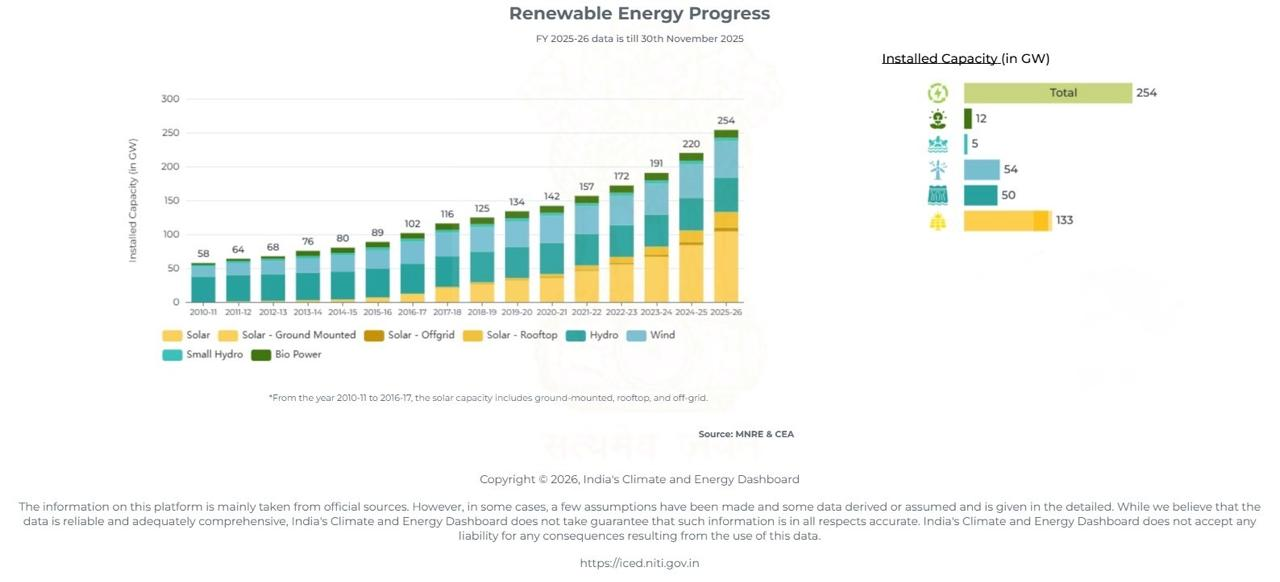
\includegraphics[width=0.65\textwidth]{image_1.jpeg} ~\cite{NITISolarIrradiance}

\end{frame}
% Slide: Comparison of Solar Water Heater Companies & PCM Usage
\begin{frame}{Comparison of Solar Water Heater Companies \& PCM Usage}

\small

% -------- Table --------
\begin{table}[h]
\centering
\renewcommand{\arraystretch}{1.1}

\resizebox{0.9\textwidth}{!}{ % adjust 0.9 -> 0.8 or 0.7 if needed
\begin{tabularx}{\textwidth}{|l|l|c|X|}
\hline
\textbf{Company} & \textbf{Country} & \textbf{PCM Used?} & \textbf{PCMs used} \\
\hline
Sunamp & UK & $\checkmark$ & Plentigrade\textsuperscript{\textregistered} PCM (main platform), P58 PCM, SU58 PCM \\
PCM Products Ltd & UK & $\checkmark$ & Positive temp (salt hydrate + organic + high-temp salts) \\
Vaillant & Germany & $\times$ & -- \\
PLUSS Advanced Technologies & India & $\checkmark$ & OM Series (Organic PCMs), FS Series (Form-stable PCMs)  \\
Chemtex Speciality Ltd & India & $\checkmark$ & Positive Temperature PCM (Heating PCM), Eutectic Salt PCM (Industrial heat management) \\
Emmvee Group & India & $\times$ & -- \\
\hline
\end{tabularx}
}
\end{table}

\vspace{0.1cm}

% -------- Conclusion --------
\textbf{Why PCM is used more in foreign countries:}

Foreign markets focus strongly on energy efficiency and carbon reduction. Government support and higher investment capacity make PCM integration commercially feasible.

\vspace{0.1cm}

\textbf{Why PCM is not widely integrated in India:}

PCM systems increase design complexity. However, with proper optimization and field validation, PCM can significantly improve hot-water availability ,sustainability and efficiency.

\end{frame}


% --- SLIDE: Motivation ---
\begin{frame}{Motivation}
\begin{itemize}
    \item Thermal energy accounts for 48--50\% of global final energy consumption. Residential water heating uses 6-8\% of household energy, underscoring SWH potential. ~\cite{duraivel2025performance}.
    \item Conventional solar water heating (SWH) systems achieve only 45--70\% annual efficiency, wasting 30--55\% of incident solar energy due to inadequate storage~\cite{AlMamun2023SWHReview}.
    \item PCM-integrated can boost thermal efficiency, can extend heat retention time and stores $\sim$50\% of total heat with $<$20\% PCM volume~\cite{Chen2025TaguchiPCM}.
    \item Global solar thermal capacity reaches $\sim$544--560 GW$_{th}$ (2024--2025); The global market for water heaters was valued at \$23.7 billion as of 2023. It is expected to reach \$32.1 billion by 2029,~\cite{OdoiYorke2025AI_SWH}.
    \item Existing PCM-SWH systems use mostly fixed/offline strategies, causing losses under variable irradiance/load; motivates. ~\cite{OdoiYorke2025AI_SWH, Chen2025TaguchiPCM}.
\end{itemize}
\end{frame}


% Slide-5: Research theme covered
\section{Research Theme}
\begin{frame}{Research Theme Covered}

\begin{columns}[T] % T = top aligned

% -------- LEFT COLUMN --------
\column{0.48\textwidth}
\textbf{Solar Energy Materials and Solar Cells}\\
\textit{Special Issue: The Use of Artificial Intelligence for Enhanced Solar Energy Harvesting and Thermal Storage}
\cite{SpecialIssueAI2026}\\
{\footnotesize (31 March 2026)}

\vspace{0.2cm}
\begin{itemize}
    \item AI for thermal energy storage systems
    \item Intelligent control of latent heat storage
    \item Machine learning--assisted material selection
    \item AI-enhanced solar thermal system performance
\end{itemize}

% -------- RIGHT COLUMN --------
\column{0.48\textwidth}
\textbf{Applied Thermal Engineering}\\
\textit{Special Issue: Next-Generation Photothermal-Driven Thermal Storage and Utilization for Buildings}
\cite{SpecialIssueATE2026}\\
{\footnotesize (17 August 2026)}

\vspace{0.2cm}
\begin{itemize}
    \item Photothermal-driven PCM thermal storage for solar applications
    \item System-level integration of thermal storage in buildings
    \item Machine learning / deep learning-based adaptive control
    \item Performance evaluation through energy efficiency analysis
\end{itemize}

\end{columns}

\end{frame}


% --- SLIDE 1: PCM-Focused ---
\section{Literature Survey}
\begin{frame}{1. Literature Survey - PCM-Focused}
\framesubtitle{Rubric: Survey Extensiveness \& Justification}
\tiny
\renewcommand{\arraystretch}{1.5}
\begin{table}
\centering
\begin{tabular}{|p{1.6cm}|p{3.0cm}|p{2.8cm}|p{3.0cm}|p{3.0cm}|}
\hline
\textbf{Author (Year)} &
\textbf{Key Objectives} &
\textbf{Parameters} &
\textbf{Methods / Models Used} &
\textbf{Future Implementations} \\
\hline
Abdulhammed K. Hamza (2025) \cite{Hamza2025PCMReview} &
Review PCM-based solar energy storage systems and assess environmental and performance impacts. &
PCM thermophysical properties, solar input, storage efficiency, lifecycle indicators. &
Literature review, Numerical modeling &
AI-assisted PCM selection, embedded optimization strategies. \\
\hline
P. K. S. Rathore (2024) \cite{Rathore2024ThermalPCM} &
Investigate PCM integration to improve solar thermal system efficiency. &
PCM type, melting range, latent heat, conductivity, storage efficiency. &
PCM integration techniques, Thermal modeling &
Advanced PCM materials, enhanced heat transfer, real-world deployment, economic analysis. \\
\hline
Franklin R.~Martinez (2025) \cite{Martinez2025PCM_Industrial} &
Evaluate PCM suitability across industrial temperature ranges. &
PCM temperature profile, stored/released energy, efficiency. &
\textbf{Differential Scanning Calorimetry (DSC)}, TGA, Thermal conductivity testing &
Long-term industrial validation and customized PCM formulations. \\
\hline

H.~E.~Abdellatif (2025) \cite{Abdellatif2025PCM_Modeling} &
Analyze design limitations and heat-transfer enhancement techniques in PCM systems. &
Thermal conductivity, latent heat, melting/solidification time, charging/discharging rate, geometry. &
\textbf{Numerical Heat Transfer Modeling}, Mathematical modeling &
Hybrid PCM systems with improved thermal conductivity and real-condition validation. \\
\hline
\end{tabular}
\end{table}
\end{frame}

% --- SLIDE 2: AI/ML in Thermal Energy Systems ---
\begin{frame}{2. Literature Survey - AI/ML in Thermal Energy Systems}
\framesubtitle{Rubric: Survey Extensiveness \& Justification}
\tiny
\renewcommand{\arraystretch}{1.5}
\begin{table}
\centering
\begin{tabular}{|p{1.6cm}|p{3.0cm}|p{2.8cm}|p{3.0cm}|p{3.0cm}|}
\hline
\textbf{Author (Year)} &
\textbf{Key Objectives} &
\textbf{Parameters} &
\textbf{Methods / Models Used} &
\textbf{Future Implementations} \\
\hline
Hayder I. Mohammed et al. (2025) \cite{Mohammed2025AIthermal} &
Analyze nanotechnology and AI approaches for enhancing thermal energy system performance. &
Nanoparticle concentration, heat transfer rate, thermal conductivity, efficiency, temperature. &
\textbf{Artificial Neural Networks (ANN)}, Optimization Algorithms &
Scalable nanomaterials, robust AI models, real-condition validation, cost optimization. \\
\hline

Artur Nem\'s (2025) \cite{Nems2025AIPCMReview} &
Review AI-driven prediction and optimization approaches for PCM thermal systems. &
Melting duration, temperature distribution, heat transfer rate, energy efficiency. &
\textbf{Machine Learning Models}, Genetic Algorithms &
Real-time AI monitoring and automated PCM selection frameworks. \\
\hline

Shuli Liu (2025) \cite{Liu2025AIPCM} &
Compare AI-based prediction with conventional thermal modeling in PCM systems. &
Solar irradiance, PCM temperature, state of charge, charging/discharging efficiency. &
\textbf{Artificial Neural Networks (ANN)}, Optimization algorithms &
Sensor-driven intelligent PCM energy management systems. \\
\hline


Peiliang Yan (2025) \cite{Yan2025ML_PCM_Melting} &
Predict melting response time of PCM in thermal energy storage systems. &
Melting time, PCM properties, geometry, operating conditions. &
\textbf{Machine Learning Regression (XGBoost)}, SVR, Random Forest &
AI predictive tools for TES design and scalable optimization. \\
\hline
\end{tabular}
\end{table}
\end{frame}

% --- SLIDE 3: AI/ML in SWH Specific ---
\begin{frame}{3. Literature Survey - AI/ML in SWH Specific}
\framesubtitle{Rubric: Survey Extensiveness \& Justification}
\tiny
\renewcommand{\arraystretch}{1.5}
\begin{table}
\centering
\begin{tabular}{|p{1.6cm}|p{3.0cm}|p{2.8cm}|p{3.0cm}|p{3.0cm}|}
\hline
\textbf{Author (Year)} &
\textbf{Key Objectives} &
\textbf{Parameters} &
\textbf{Methods / Models Used} &
\textbf{Future Implementations} \\
\hline
Flavio Odoi-Yorke (2025) \cite{OdoiYorke2025AI_SWH} &
Review AI applications in solar water heating systems. &
Solar radiation prediction, system efficiency, control variables. &
\textbf{Artificial Neural Networks (ANN)}, Machine Learning, Predictive analytics &
Hybrid AI--PCM integration, intelligent predictive control for SWH systems. \\
\hline
A. O. Eldokaishi (2022) \cite{Eldokaishi2022ANN_PCM_SWH} &
Model PCM-integrated solar water heating system using ANN-based prediction. &
Water temperature, PCM phase change behavior, solar input, storage performance. &
\textbf{Artificial Neural Networks (ANN)}, Numerical modeling &
Advanced ANN-based supervisory thermal control. \\
\hline

Ehsanolah Assareh (2023) \cite{Assareh2023ML_PCM_SolarCollector} &
Improve PCM-enhanced solar collectors using ML-driven multi-objective optimization. &
Collector efficiency, PCM properties, thermal output, operating temperature. &
\textbf{Machine Learning-based Multi-objective Optimization}, Comparative performance analysis &
Climate-adaptive AI optimization frameworks for solar collectors. \\
\hline 

Muthanna (2025) \cite{MJET2025PCM} &
Develop ML-based controller for PCM-integrated solar water heating systems. &
Phase dynamics, flow rate, environmental conditions, heat transfer. &
\textbf{Artificial Neural Network (ANN)}, Dynamic simulation &
Retrofit AI control for existing systems without hardware changes. \\
\hline
\end{tabular}
\end{table}
\end{frame}

% --- SLIDE 4: Climate Integrated in PCM in SWH ---
\begin{frame}{4. Literature Survey - Climate Integrated in PCM in SWH}
\framesubtitle{Rubric: Survey Extensiveness \& Justification}
\tiny
\renewcommand{\arraystretch}{1.5}
\begin{table}
\centering
\begin{tabular}{|p{1.6cm}|p{3.0cm}|p{2.8cm}|p{3.0cm}|p{3.0cm}|}
\hline
\textbf{Author (Year)} &
\textbf{Key Objectives} &
\textbf{Parameters} &
\textbf{Methods / Models Used} &
\textbf{Future Implementations} \\
\hline
Brihaspati Singh (2025) \cite{Singh2025PCMSWH} &
Review PCM storage techniques for improving solar water heating performance. &
Hot-water temperature, PCM melting range, storage capacity. &
ETC integration, Storage modeling &
Climate-specific optimization and adaptive PCM control strategies. \\
\hline
Fangcheng Kou (2025) \cite{Kou2025BIHPPCM} &
Integrate PCM with heat pipes for enhanced solar heating and storage efficiency. &
Phase change enthalpy, phase change temperature, thermal conductivity. &
Numerical heat-transfer modeling, \textbf{Heat Pipe--PCM integration model} &
Further thermal performance optimization across climates. \\
\hline
Emami et al. (2026) \cite{Emami2026DRLSolar} &
Develop intelligent control for solar-driven power cycle with thermal energy storage. &
Thermal storage state, solar irradiance, load demand, control actions. &
\textbf{Deep Reinforcement Learning (DRL)}, Case study simulation &
Real-time AI-based TES control, grid-interactive solar thermal systems. \\
\hline
Guan-Rong Chen (2025) \cite{Chen2025TaguchiPCM} &
To optimize parameter design of integrated solar water heating systems using PCM for improved heat retention. &
PCM material, PCM volume, tube configuration, working fluid, collector tubes, absorber plate. &
Taguchi orthogonal array design, signal-to-noise analysis, main effects analysis. &
Incorporating fins in PCMs or heat pipes for faster charging/discharging and enhanced performance. \\
\hline
\end{tabular}
\end{table}
\end{frame}

% --- SLIDE 5: Broader Advanced Topics ---
\begin{frame}{5. Literature Survey - Broader Advanced Topics}
\framesubtitle{Rubric: Survey Extensiveness \& Justification}
\tiny
\renewcommand{\arraystretch}{1.5}
\begin{table}
\centering
\begin{tabular}{|p{1.6cm}|p{3.0cm}|p{2.8cm}|p{3.0cm}|p{3.0cm}|}
\hline
\textbf{Author (Year)} &
\textbf{Key Objectives} &
\textbf{Parameters} &
\textbf{Methods / Models Used} &
\textbf{Future Implementations} \\
\hline
Rajamurugu N. (2025) \cite{Rajamurugu2025PCMML} &
Enhance PCM-based system performance using machine learning techniques. &
PCM properties, thermal efficiency, ambient temperature. &
\textbf{Multi-Layer Perceptron (MLP)}, Random Forest, Support Vector Regression (SVR) &
ML-based performance estimation; lacks embedded real-time control. \\
\hline 

Abdelkrim Terfai et al. (2025) \cite{Terfai2025SolarPond_ANN_MPC} &
Improve thermal prediction and control of solar pond storage system. &
Heat extraction mode, temperature stratification, solar irradiance, storage behavior. &
\textbf{Model Predictive Control (MPC)}, Artificial Neural Network (ANN) &
Scalable AI-driven thermal storage control for hybrid solar systems. \\
\hline

Mohammad Saleh Barghi (2025) \cite{Barghi2026SolarDryingPCM} &
Optimize PCM-assisted solar drying systems using AI-based performance prediction. &
PCM melting temperature, solar radiation, air temperature, drying time, efficiency. &
\textbf{Artificial Neural Networks}, Support Vector Machine, Evolutionary Polynomial Regression &
Real-time AI control and large-scale smart drying systems. \\
\hline

Mohammad Hasan Ghodusinejad (2025) \cite{Ghodusinejad2026SolarForecast} &
Review and compare solar irradiance forecasting techniques. &
Solar irradiance, forecast horizon, meteorological variables, cloud cover. &
\textbf{AI-based Forecasting Models}, Numerical Weather Prediction (NWP), Hybrid models &
Physics-informed AI and real-time adaptive forecasting systems. \\
\hline 

\end{tabular}
\end{table}
\end{frame}


%--Research Gaps--%
\begin{frame}{Research Gaps}
\small
\begin{enumerate}
    \item \textbf{Limited real-time adaptive control:}
    Most PCM-based systems use passive or fixed-rule strategies, lacking dynamic response to varying solar input and demand~\cite{Hamza2025PCMReview, Singh2025PCMSWH}.
    \item \textbf{Lack of integrated PCM--AI--hardware systems:}
    Prior studies treat materials, control, and implementation separately without a complete working prototype~\cite{Chen2025TaguchiPCM, Liu2025AIPCM, Nems2025AIPCMReview}.
    \item \textbf{Poor alignment with real usage patterns:}
    Existing systems rarely adapt storage and release based on actual household demand~\cite{Hamza2025PCMReview, Singh2025PCMSWH}.
    \item \textbf{Limited real-world validation:}
    Most research relies on simulations or short-term tests rather than long-term experimental evaluation~\cite{Hamza2025PCMReview, Abdellatif2025PCM_Modeling}.
    \item \textbf{Limited predictive optimization under climatic uncertainty:}
    Most PCM-based systems lack predictive models to anticipate variations in solar input and demand, leading to suboptimal thermal storage utilization~\cite{Hamza2025PCMReview, Nems2025AIPCMReview, Liu2025AIPCM}.
\end{enumerate}
\end{frame}



% --- SLIDE 12: ORIGINALITY (Rubric: 4 Marks) Objectives---
\section{Objectives}
\begin{frame}{Objectives}
\begin{block}{Overall Problem}
Most PCM-based solar water heating systems use passive or fixed control rules, 
leading to delayed heat availability, inefficient storage, and energy loss 
under variable solar and demand conditions.
\end{block}

\begin{itemize}

    \item  Collect and process climate data and thermal parameters data to classify and select the most suitable PCM for forecasted climate and demand conditions.(RG 2, RG 5)

    \item Train a DRL agent to adaptively control PCM charge, discharge, and bypass modes to maximise hot-water availability. (RG 1, RG 3, RG 5)

    \item Build a thermal simulation as the DRL training environment and benchmark the controller against rule-based and passive baselines. (RG 1, RG 4)

    \item Deploy the AI controller on embedded hardware as a closed-loop prototype 
    and evaluate performance across Indian climate profiles. (RG 2, RG 3, RG 4)

\end{itemize}

\end{frame}

\begin{comment}
\begin{frame}{Objectives (detailed)}
\begin{itemize}

    \item Collect and process real-time multi-sensor data to classify and select the 
    most thermally suitable PCM for prevailing climatic and demand conditions using 
    a trained ML model. (RG 2, RG 5)

    \item Design and train a Deep Reinforcement Learning (DRL) agent to adaptively 
    regulate PCM charge, discharge, and bypass modes in real time, maximising 
    hot-water availability under varying solar irradiance and household demand 
    profiles. (RG 1, RG 3, RG 5)

    \item Develop a physics-informed grey-box thermal simulation of the PCM storage 
    unit to serve as the DRL training environment, and benchmark the trained 
    controller against rule-based and passive baselines using defined thermal 
    performance metrics. (RG 1, RG 4)

    \item Deploy the validated AI controller on an embedded Raspberry Pi platform as 
    a fully autonomous closed-loop prototype, and experimentally evaluate hot-water 
    yield and thermal efficiency across multiple Indian climate profiles. (RG 2, RG 3, RG 4)

\end{itemize}
\end{frame}
\end{comment}
 

%Slide 13:Problem Statement
% --- SLIDE: PROBLEM STATEMENT (DESIGN STYLE) ---

% --- Problem Description ---
\section{Problem Statement}
\begin{frame}{Problem Statement}

% --- Problem Description ---
\vspace{0.3cm}

% --- Core Problem Block ---
\begin{block}{Novel Idea}
To design and implement an autonomous, AI-driven PCM-based thermal storage system that dynamically optimizes heat charging and discharging under real-world operating conditions.
\end{block}

\vspace{0.4cm}

% --- Sustainability Heading ---
\textbf{Sustainable Development Goals related to the problem:}

\vspace{0.3cm}

% --- SDG ICONS ROW ---
\begin{center}
\begin{tabular}{c c c c}
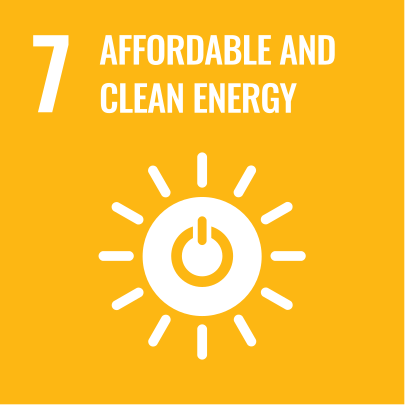
\includegraphics[width=2.2cm]{7.png} &

\includegraphics[width=2.2cm]{9.png} &
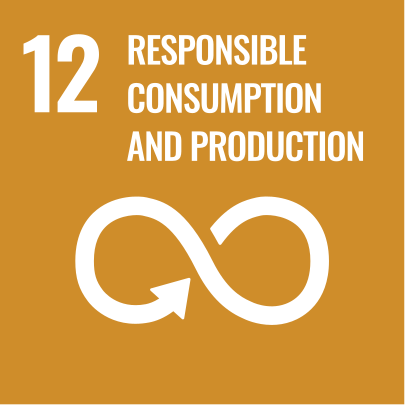
\includegraphics[width=2.2cm]{12.png} &
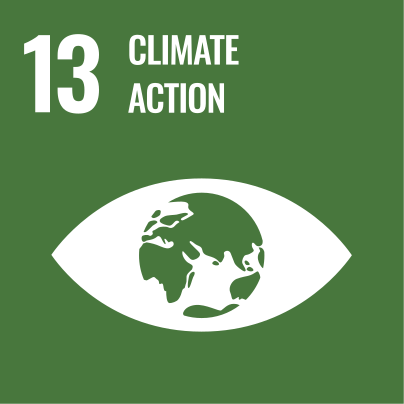
\includegraphics[width=2.2cm]{13.png}
\end{tabular}
\end{center}

\end{frame}


%Slide 16-Total Architecture
\section{Architecture}
\begin{frame}{Proposed Architecture Diagram}
    \begin{figure}
        \centering
        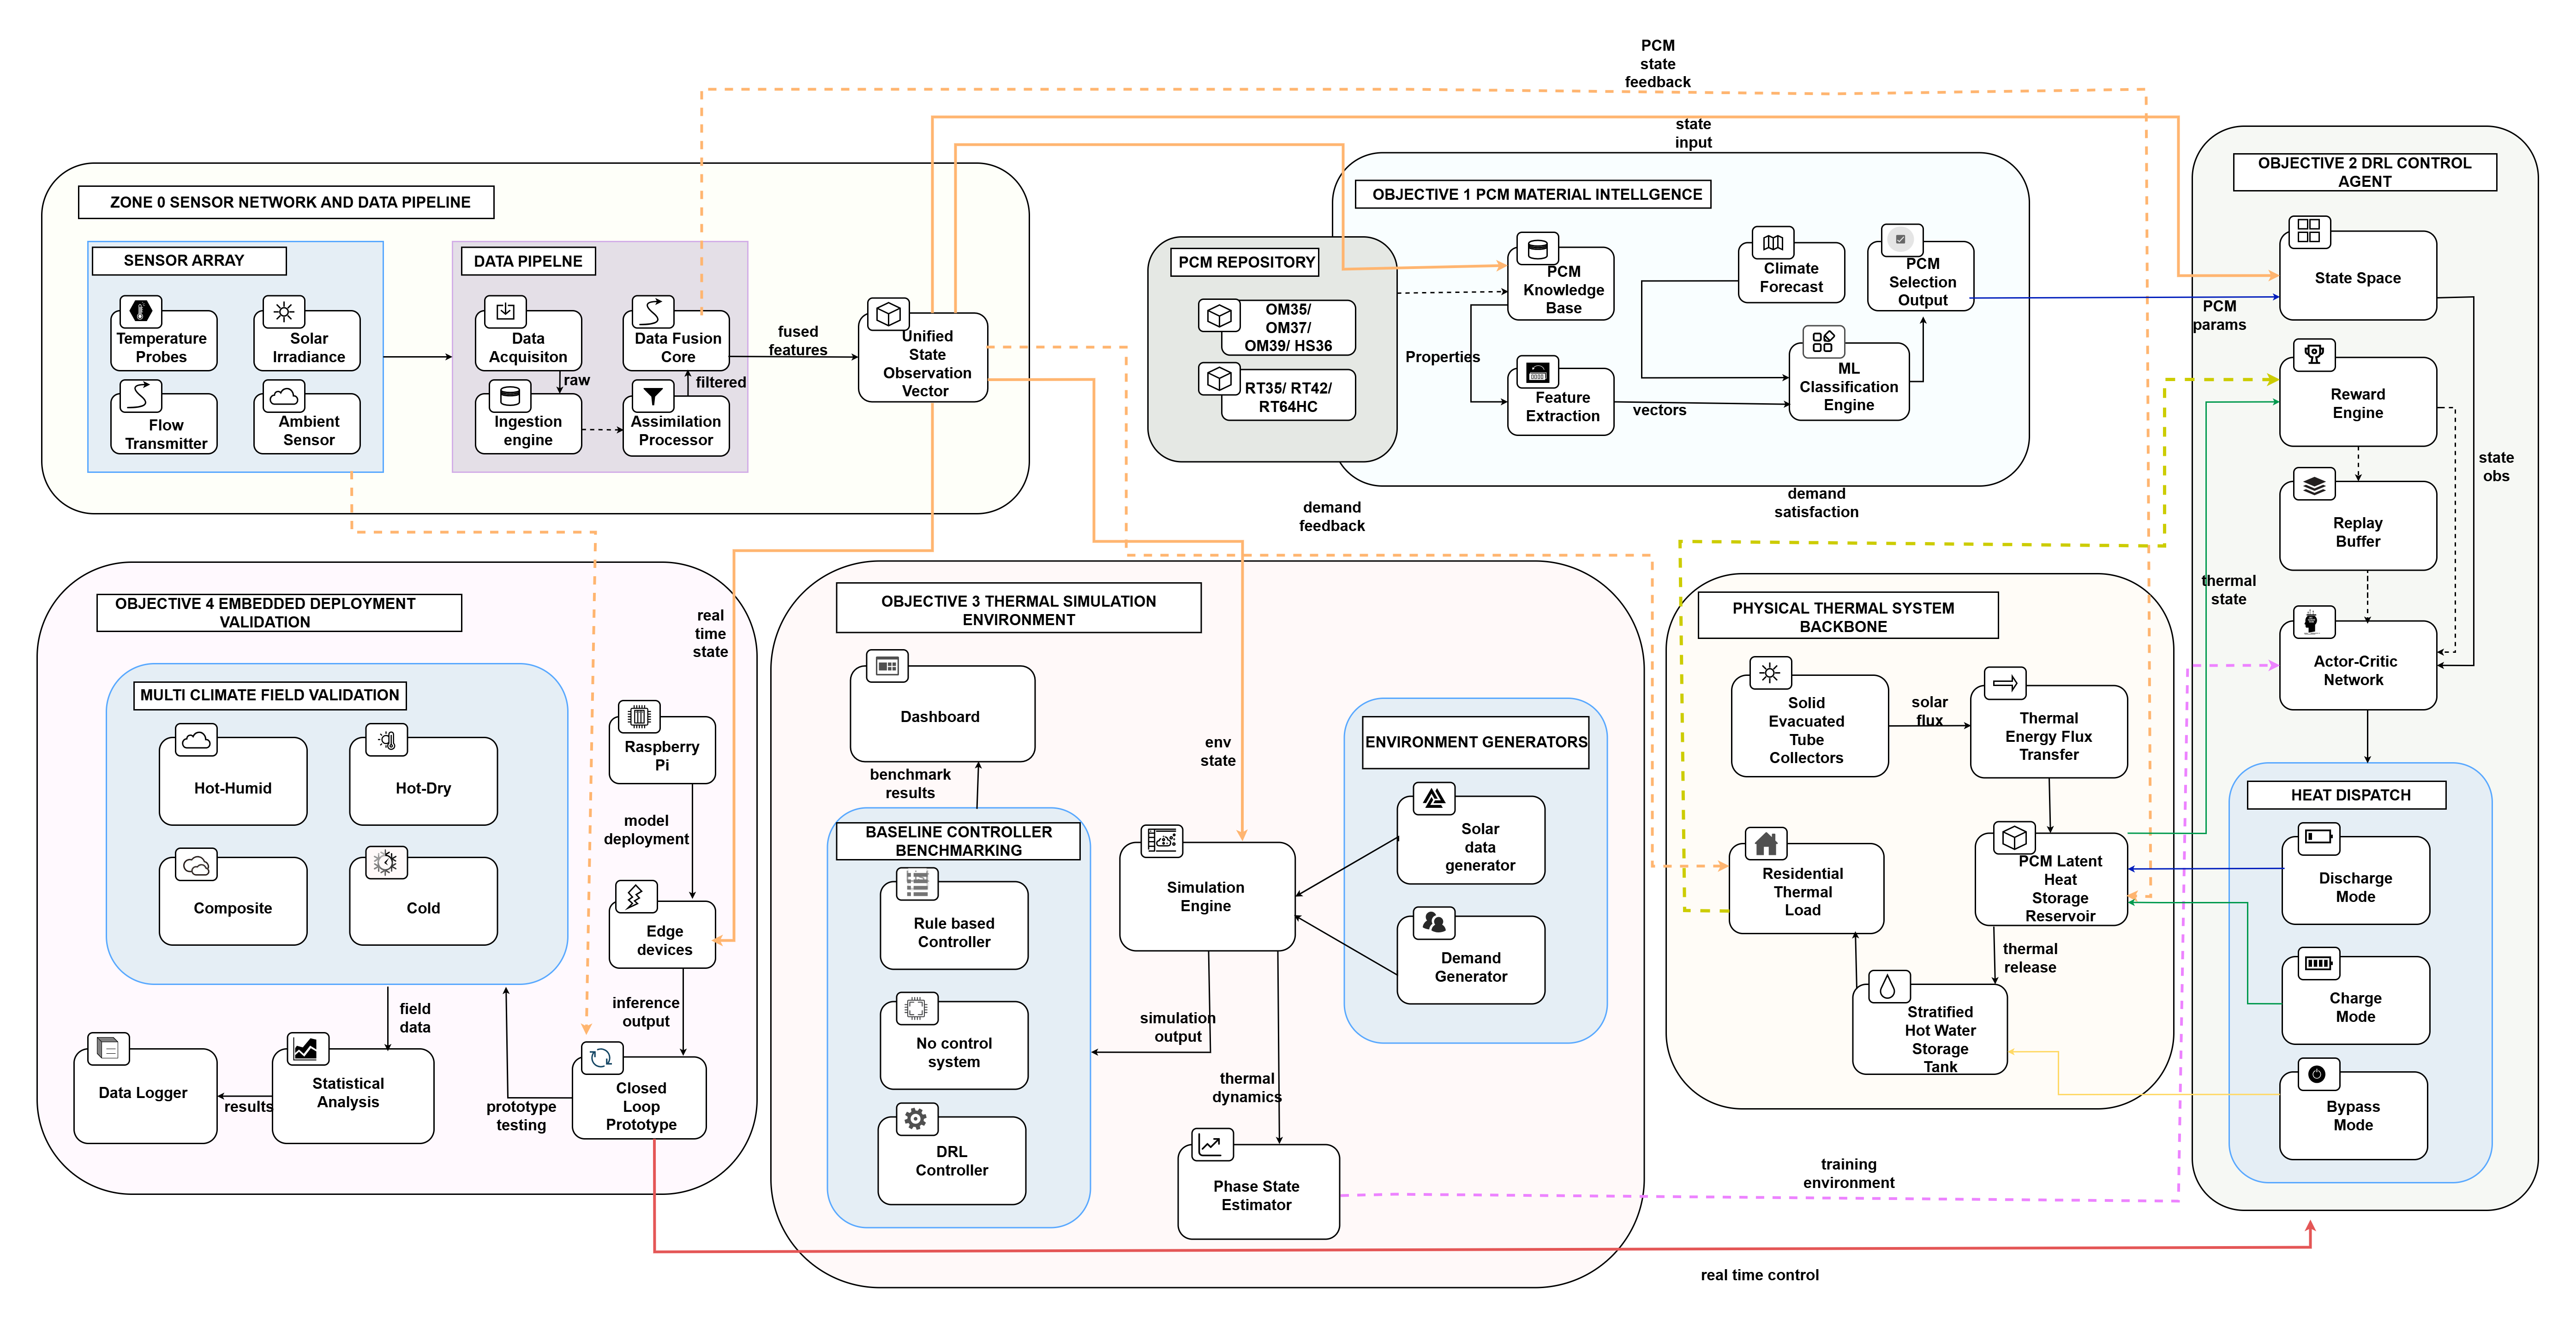
\includegraphics[width=1.0\textwidth]{architecture.png}
    \end{figure}
\end{frame}

%Slide 16-Architecture Diagram of Objective 1
\section{Architecture}
\begin{frame}{Architecture Diagram of Objective 1}
    \begin{figure}
        \centering
        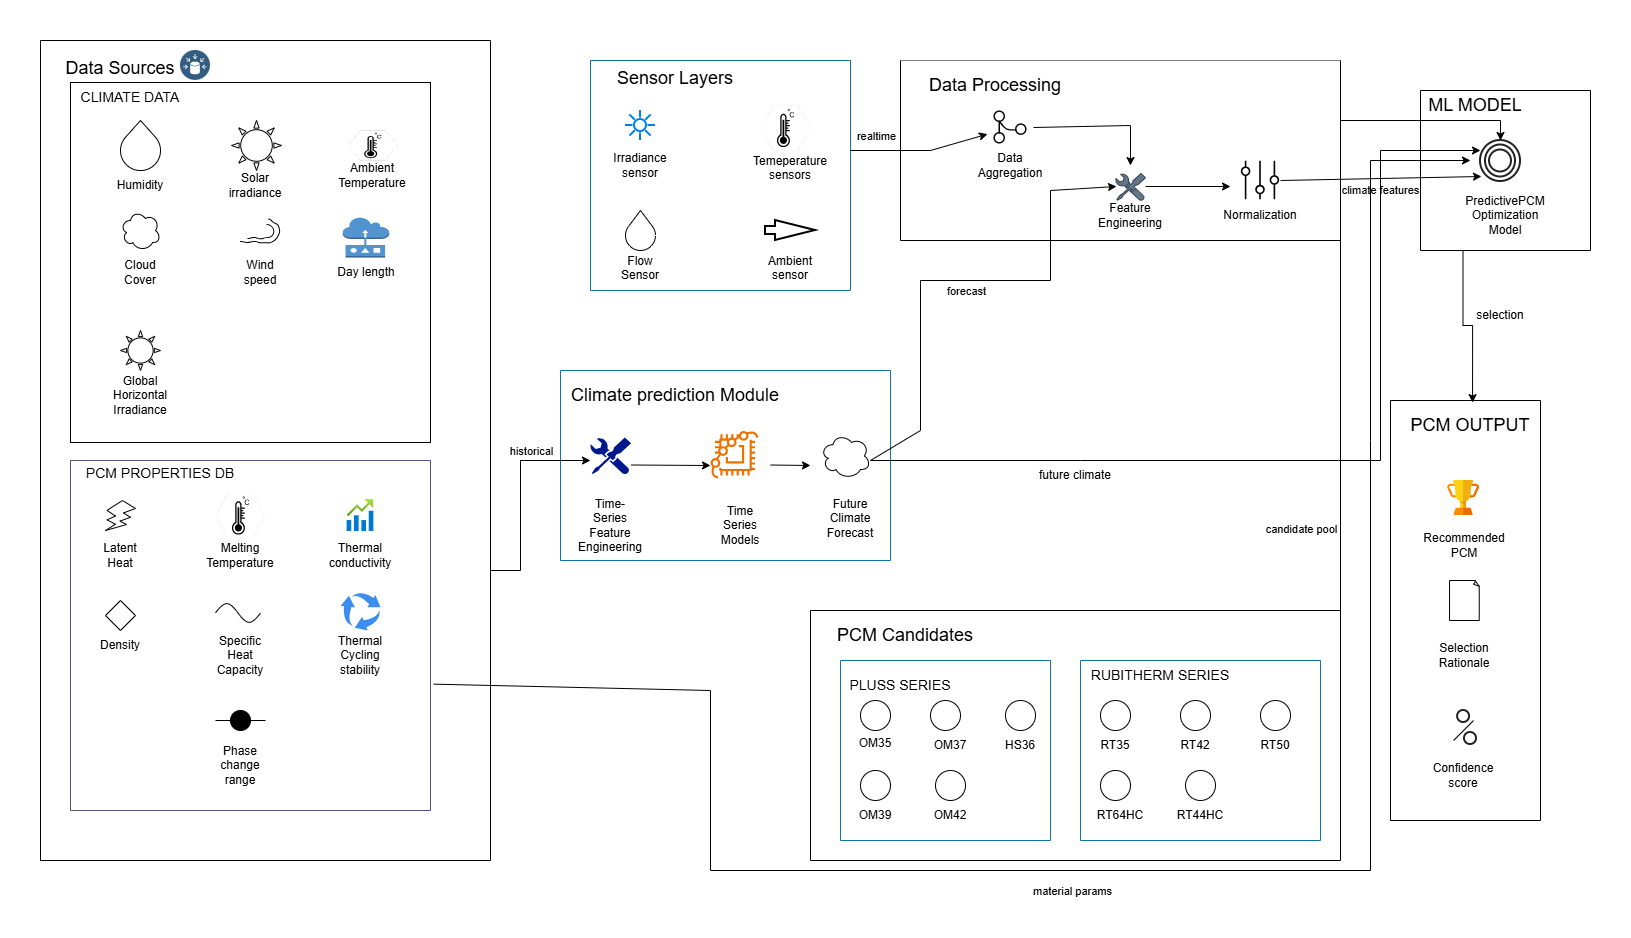
\includegraphics[width=0.95\textwidth]{obj_1.png}
    \end{figure}
\end{frame}

\section{Technical Knowledge}
% -------------------- Slide 1 --------------------
\begin{frame}{Technical Knowledge --- PCM Selection Methodology (Objective 1)}
\small

\textbf{Mapped Objective:} Optimal PCM selection under climate conditions

\vspace{0.2cm}
\textbf{Climate \& PCM Data Integration:}
Climate data and PCM material properties are integrated using a Machine Learning model to predict thermal performance under forecasted climate conditions.

\vspace{0.3cm}
\textbf{Taguchi Method:}\cite{Chen2025TaguchiPCM}
\begin{itemize}
    \item Statistical Design of Experiments method using orthogonal arrays.
    \item Used to determine optimal combination of PCM properties affecting thermal performance.
\end{itemize}

\vspace{0.3cm}
\textbf{Grey Relational Analysis (GRA):}
\begin{itemize}
    \item Multi-criteria decision-making method.
    \item Used to rank PCM materials based on thermal performance.
\end{itemize}

\end{frame}

% -------------------- Slide 2 --------------------
\begin{frame}{Technical Knowledge --- PCM Selection Criteria and GRG}
\small
\textbf{Selection Criteria:} The PCM is selected based on melting temperature suitability, latent heat, thermal conductivity, and overall heat storage capacity under given climate conditions.

\vspace{0.2cm}
\textbf{Grey Relational Grade (GRG):}
\[
\gamma_i = \frac{1}{n} \sum \xi_i
\]

\[
\xi_i = \frac{\Delta_{\min} + \zeta \Delta_{\max}}{\Delta_i + \zeta \Delta_{\max}}
\]

\vspace{0.2cm}
\textbf{Output:}
\begin{itemize}
    \item GRG calculated for each PCM
    \item PCM ranked based on GRG
    \item PCM with highest GRG selected as optimal PCM
\end{itemize}

\end{frame}

%Slide 16-Architecture Diagram of Objective 2
\section{Architecture}
\begin{frame}{Architecture Diagram of Objective 2}
    \begin{figure}
        \centering
        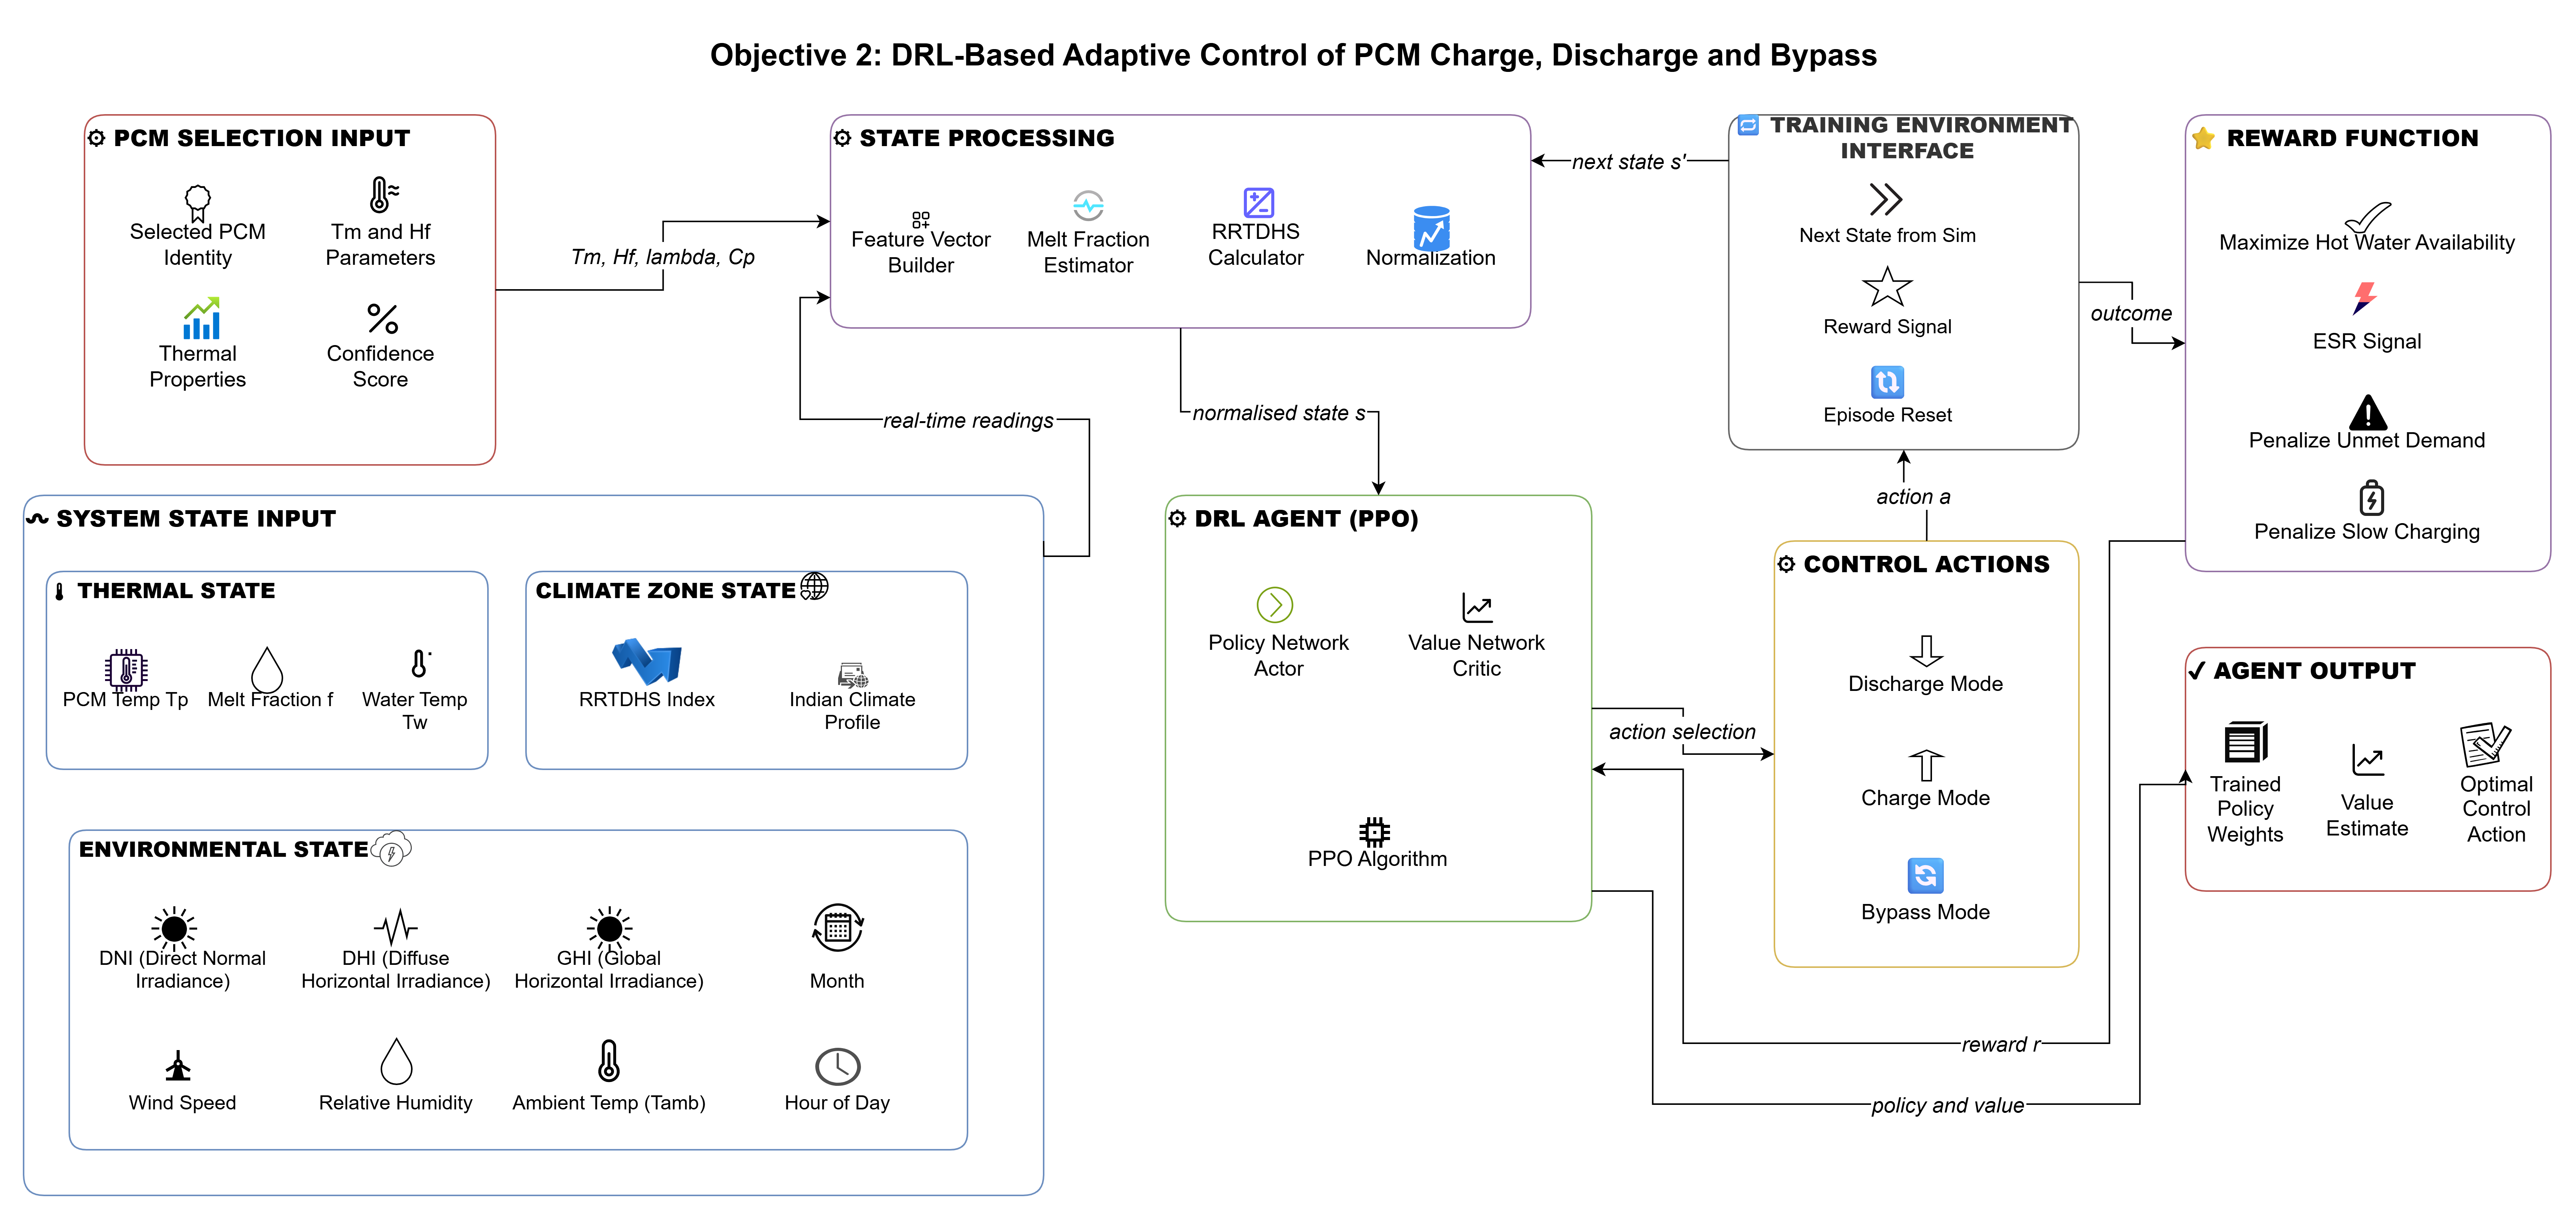
\includegraphics[height=0.85\textheight]{obj_2.png}
    \end{figure}
\end{frame}

% -------------------- Slide 3 --------------------
\begin{frame}{Technical Knowledge --- AI-Based Control (Objective 2)}
\small

\textbf{Mapped Objective:} DRL-based adaptive control of PCM charge, discharge, and bypass

\vspace{0.2cm}
\textbf{DRL:} Learns optimal control policy under dynamic thermal and solar conditions

\vspace{0.2cm}
\textbf{State:} $s_t = [T_w,\ T_p,\ f,\ GHI,\ T_{amb},\ wind,\ time]$

\vspace{0.2cm}
\textbf{Actions:} Charge, Discharge, Bypass

\vspace{0.2cm}
\textbf{Environment:} Grey-box thermal model (generates next state $s_{t+1}$)

\vspace{0.2cm}
\textbf{Reward:} Maximizes hot-water availability + energy reliability (ESR) \\
\hspace{1.6cm} penalizes unmet demand and slow charging

\vspace{0.2cm}
\textbf{Agent:} Actor--Critic (Policy Network + Value Network)

\vspace{0.2cm}
\textbf{Algorithm:} PPO (Proximal Policy Optimization)

\end{frame}
%Slide 16-Architecture Diagram of Objective 3 and 4
\section{Architecture}
\begin{frame}{Architecture Diagram of Objective 3 and 4}
    \begin{figure}
        \centering
        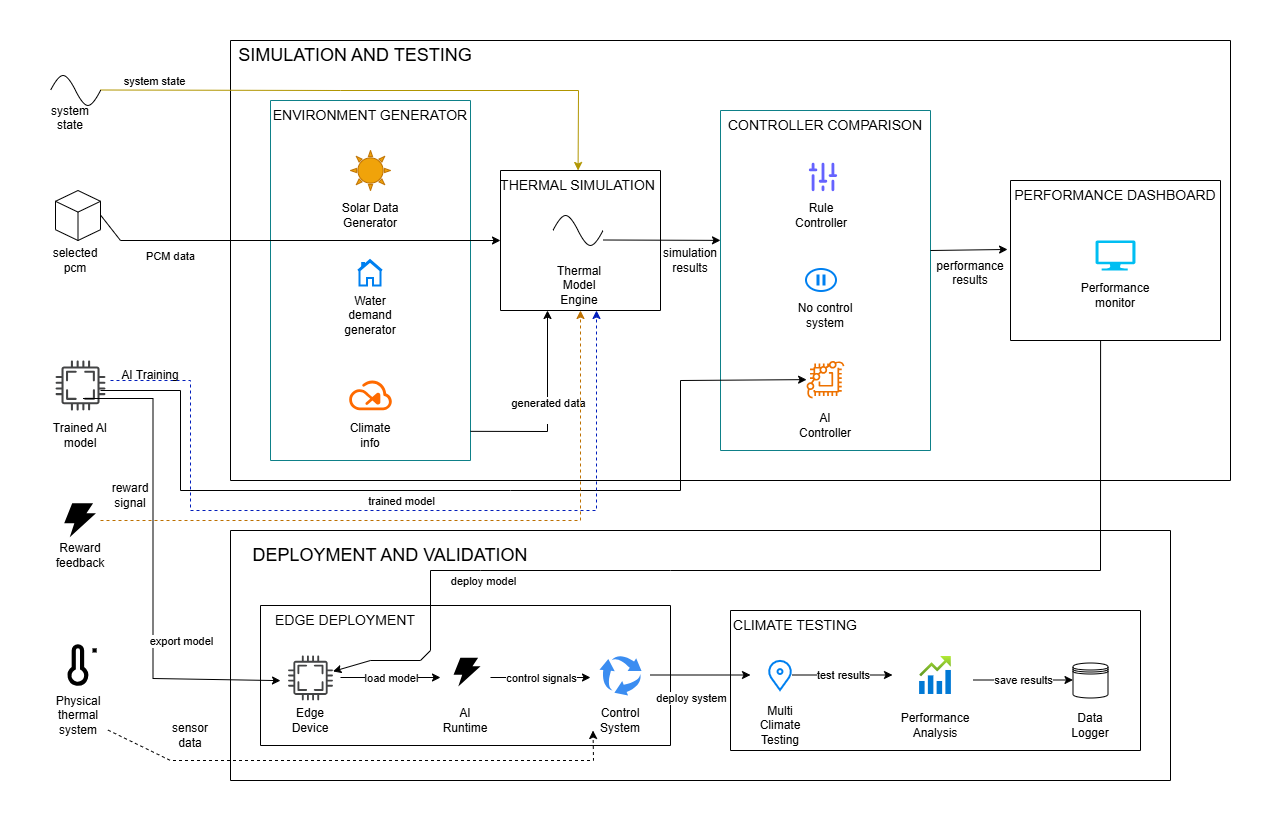
\includegraphics[height=0.95 \textheight]{obj_34.png}
    \end{figure}
\end{frame}


% Slide 17: Data Sets
\section{Data Collection}
% -------------------- Slide 17.1 --------------------
\subsection{PCM Characterization and Properties}
\begin{frame}{Data Collection --- PCM Properties}
\begin{itemize}

    \item Selection criteria follow the priority ranking established by 
    Singh~et~al.~\cite{Singh2025PCMSWH}: latent heat $\rightarrow$ thermal 
    conductivity $\rightarrow$ melting temperature $\rightarrow$ specific heat 
    $\rightarrow$ density.

    \item Target operating range for solar water heating: \textbf{$T_m$ = 
    35--65\,\textdegree C}, validated across multiple SWH studies 
    \cite{Singh2025PCMSWH, Chen2025TaguchiPCM}.

    \item \textbf{Rubitherm RT Series} \cite{RubithermPCM} --- commercial 
    paraffin-based PCMs:
    \begin{itemize}
        \item RT35, RT38\,HC, RT42, RT44\,HC, RT45\,HC, RT47, RT50, 
              RT54\,HC, RT55, RT64\,HC
        \item Pre-engineered for higher $\lambda$; rated safe for domestic 
              applications
    \end{itemize}

    \item \textbf{PLUSS savE\textsuperscript{\textregistered} / OM Series} 
    \cite{PlussPCM} --- bio-based organics suited to Indian supply chains:
    \begin{itemize}
        \item savE\,HS36, OM35, OM37, OM39, OM42, OM46, OM48, OM50
    \end{itemize}

    \item Eutectic blends (e.g., Lauric--Myristic 66/34, $T_m$ = 34.2\,\textdegree C) 
    provide tunable $T_m$ for climate-zone-specific recommendation 
    \cite{Singh2025PCMSWH}.
    \item Climate data drives both the \textbf{PCM classifier state vector} 
    and the \textbf{PPO agent's observation space}:
    $\mathbf{s} = [\text{GHI, DNI, }T_{\text{amb}}\text{, }
    v_{\text{wind}}\text{, RH, Hour, Month, }
    T_{\text{PCM}}\text{, }T_w\text{, }f_{\text{melt}}\text{, 
    Demand}]$~\cite{Liu2025AIPCM}.
\end{itemize}
\end{frame}


% -------------------- Slide 17.3 --------------------
\subsection{Solar Irradiance and Weather Inputs}
\begin{frame}{Data Collection --- Solar and Environmental Data}
\begin{itemize}


    \item \textbf{ERA5 Reanalysis (Copernicus / ECMWF)} \cite{ERA5} --- 
    primary multi-year climate backbone:
    \begin{itemize}
        \item \texttt{GHI} (surface solar radiation downwards), 
              \texttt{DNI} (direct normal irradiance), 
              \texttt{DHI} (diffuse horizontal irradiance),total cloud cover, surface pressure, relative humidity
        \item Hourly resolution; used to compute clear-sky index 
              $K_c = \text{GHI}/\text{GHI}_\text{clear}$ 
              \cite{Ghodusinejad2026SolarForecast}
    \end{itemize}

    \item \textbf{NASA POWER Data Access Viewer} \cite{NASAPOWER} --- 
    validated solar resource data at 0.5\textdegree\ resolution for Indian cities (eg : Coimbatore, Kochi):
    \begin{itemize}
        \item GHI, DNI, DHI, $T_\text{amb}$, wind speed, humidity\ feature vector 
    \end{itemize}

    \item \textbf{ISRO Solar Energy Calculator} \cite{ISROSolarCalculator}, 
    \textbf{Global Solar Atlas} \cite{GlobalSolarAtlasIndia} --- used to 
    cross-validate GHI estimates and derive the climate suitability index:
    \[
      \text{RRTDHS} = \frac{\bar{Q}_\text{sol}}{T_\text{set} - 
      \bar{T}_\text{out}} \quad \text{\cite{Kou2025BIHPPCM}}
    \]

    \item Sensor resolution benchmark: $\pm$0.2\,\textdegree C (temperature), 
    $\pm$10\,W/m\textsuperscript{2} (irradiance), 60\,s interval --- 
    consistent with DS18B20 + pyranometer hardware\ \cite{Kou2025BIHPPCM}.
\end{itemize}
\end{frame}

% ====================== APPENDIX SLIDE ======================
\section{Appendix}
\begin{frame}{Appendix: Data Preprocessing Visualizations}
\centering

\begin{tabular}{cc}
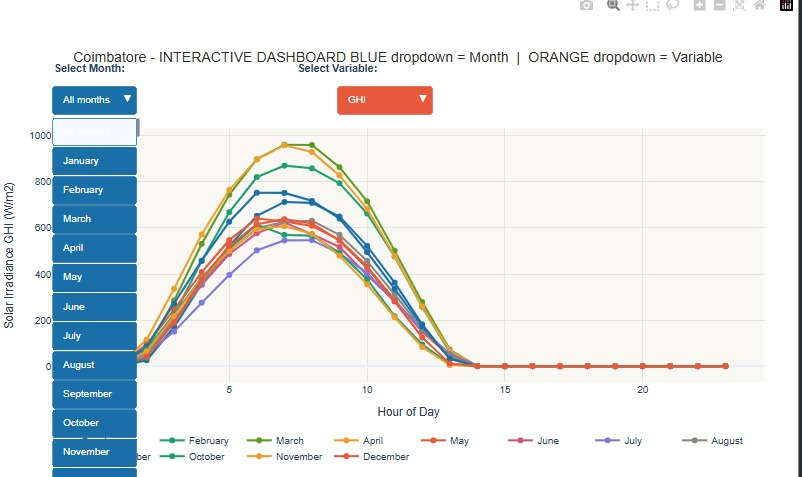
\includegraphics[width=0.45\textwidth,height=0.38\textheight,keepaspectratio]{graph1.jpeg} &
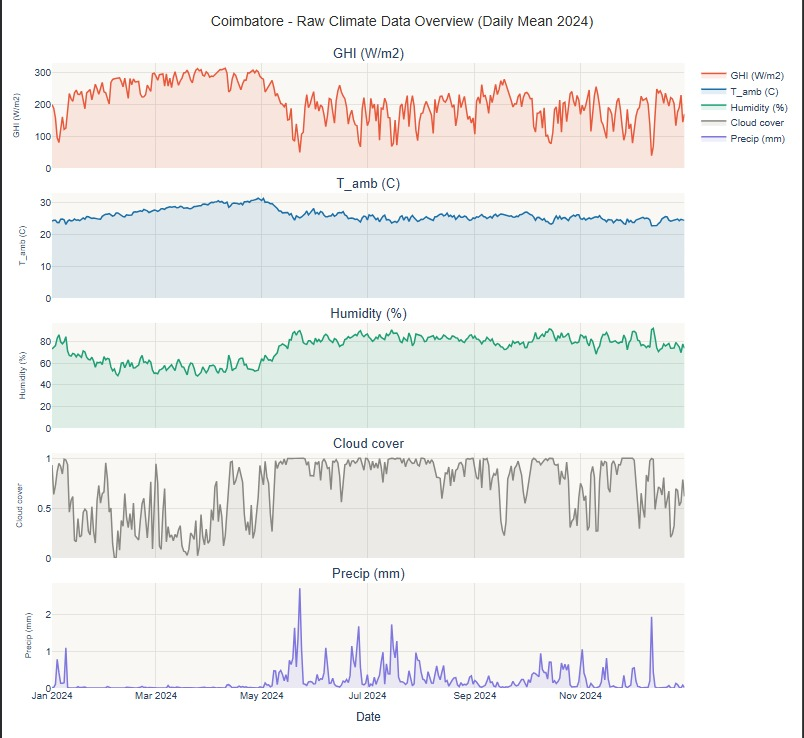
\includegraphics[width=0.45\textwidth,height=0.38\textheight,keepaspectratio]{graph2.jpeg} \\[4pt]

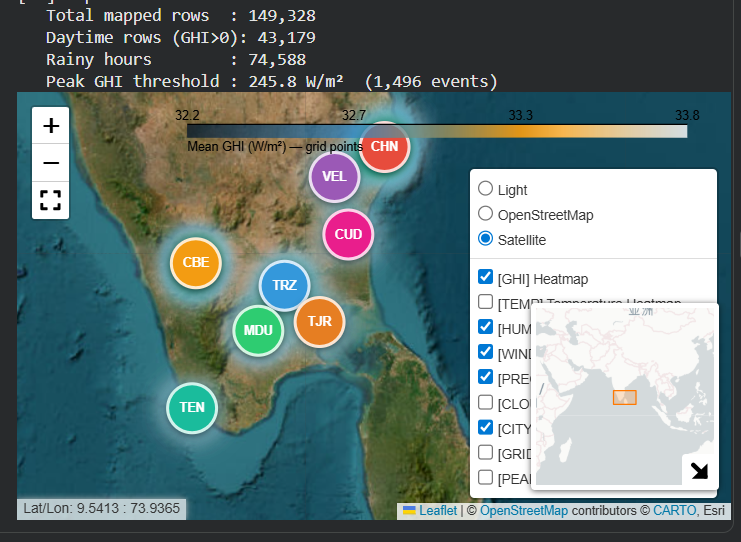
\includegraphics[width=0.45\textwidth,height=0.38\textheight,keepaspectratio]{map_interactive.png} &
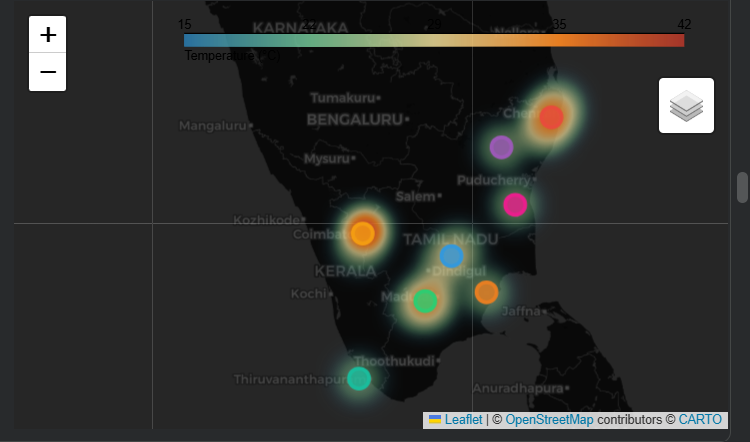
\includegraphics[width=0.45\textwidth,height=0.38\textheight,keepaspectratio]{irridiance.png}
\end{tabular}

\vspace{0.1cm}
\small
\textbf{Top row:} Feature distributions \& correlation matrix (post-scaling)  
\textbf{Bottom row:} Spatial coverage map\& irradiance time-series example \cite{ERA5}, \cite{NASAPOWER}, \cite{ISROSolarCalculator}, \cite{GlobalSolarAtlasIndia}

\end{frame}

% --- REFERENCES ---
\section{References}
\begin{frame}[allowframebreaks]{References}
 \tiny
    \bibliographystyle{IEEEtran}
    \bibliography{references} 
\end{frame}


% --- THANK YOU ---
\begin{frame}
    \centering    
    {\Huge \textbf{\textcolor{amritaMaroon}{Thank You}}}
\end{frame}

\end{document}